\subsubsection{Encryption - Action Obfuscator} \label{subsubsectionection:counter-replace-encryption-content-obfuscator}
The second approach is to use encryption as obfuscation.
The idea is to have a single method to deligate all other method calls according to an encrypted parameter.
\newline
When an attacker does a static analysis of the code, the links between method call and executing method are not apparent.
It forces the attacker to use a dynamic analysis method instead.
The fortification of the mechanism is improved when encrypted arguments are passed as well and the decryption is done in the executing method.
This requires more than just opcodes to be circumvented.
\newline
An abstract presentation of the mechanism can be seen in figure~\ref{fig:encryptionAction}.
\begin{figure}[h]
    \centering
    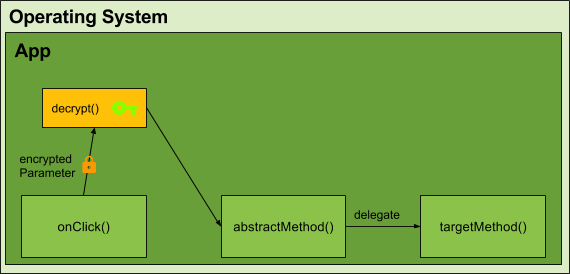
\includegraphics[width=0.8\textwidth]{data/encryptionAction.png}
    \caption{Encrypted actions to obfuscate dependencies}
    \label{fig:encryptionAction}
\end{figure}
